\chapter{Parameter analysis}
\section{open questions}
\begin{enumerate}
        \item Analysis of detection rate for fully relativistic model.
        \item how do we precisely measure the MBH mass if red shifted mass is accurate but luminal distance has 10\% error.
\end{enumerate}


\section{FEW package}
Provides EMRI waveforms using fully relativistiv Schwarzschild or the \emph{Augumented Analytic Kludge} model.

\subsection{Kludge model}
Contrasting with the slow gravitational self-force wave-
form models are the fast EMRI “kludge” models which
are designed to be rapidly evaluated for use in LISA data
analysis studies [30–33]. These models capture the phe-
nomenology of generic EMRI waveforms but only have
an approximation to the correct phasing and amplitudes.
They achieve this by computing the inspiral using (post-
Newtonian inspired) analytic fits to pieces of the gravi-
tational self-force and then approximating the waveform
using a “semi-relativistic” quadrupole formula (possibly
with octupolar corrections [31]). This weak-field approx-
imation fundamentally limits the improvements that can
be made to these models. Nonetheless, kludge mod-
els are currently the only EMRI templates available for
use in data analysis studies that encompass the full 14-
dimensional parameter space of EMRIs (neglecting the
spin of the secondary). For this reason they are the only
EMRI models to have been used so far in LISA data
analysis studies [34, 35].


\section{EMRI with LISA paper}
\emph{EMRI with LISA} analyzes the EMRI count, waveforms, signal analysis and parameter estimations. They evaluate this for the \emph{Analytic Kludge} (AK) model for \emph{Schwarzschild} (AKS) and \emph{Kerr} (AKK).

\subsection{detection rate}
AKS $\approx 10\% $\\
AKK $\approx 10\% - 20\%$

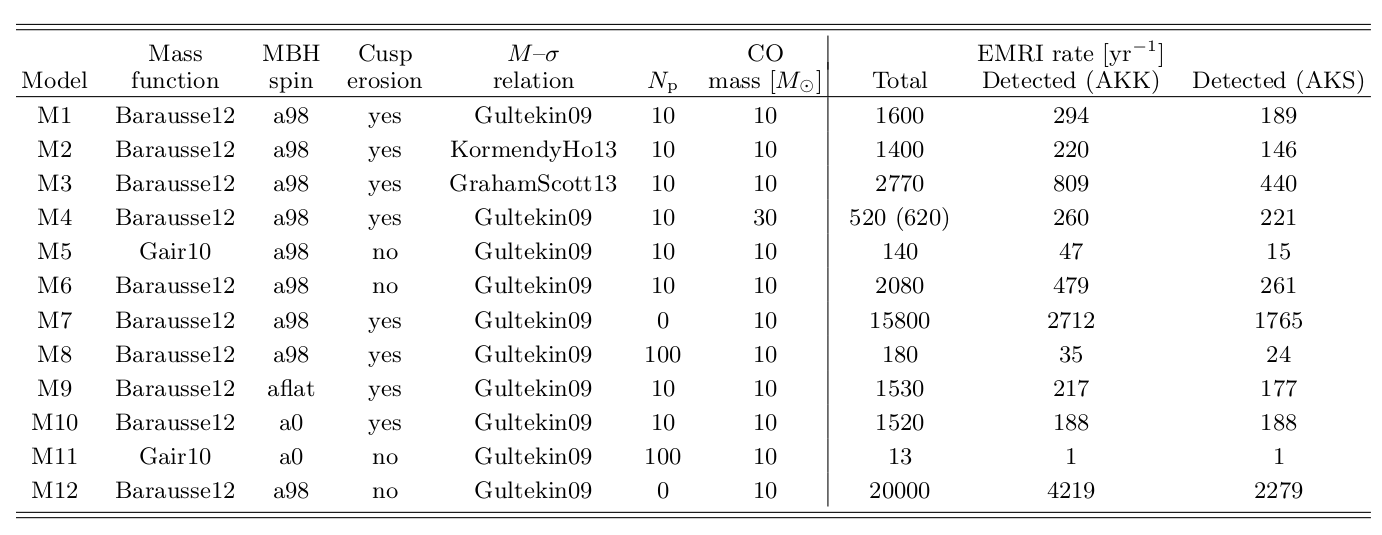
\includegraphics[width=\textwidth]{img/detection_rates.png}

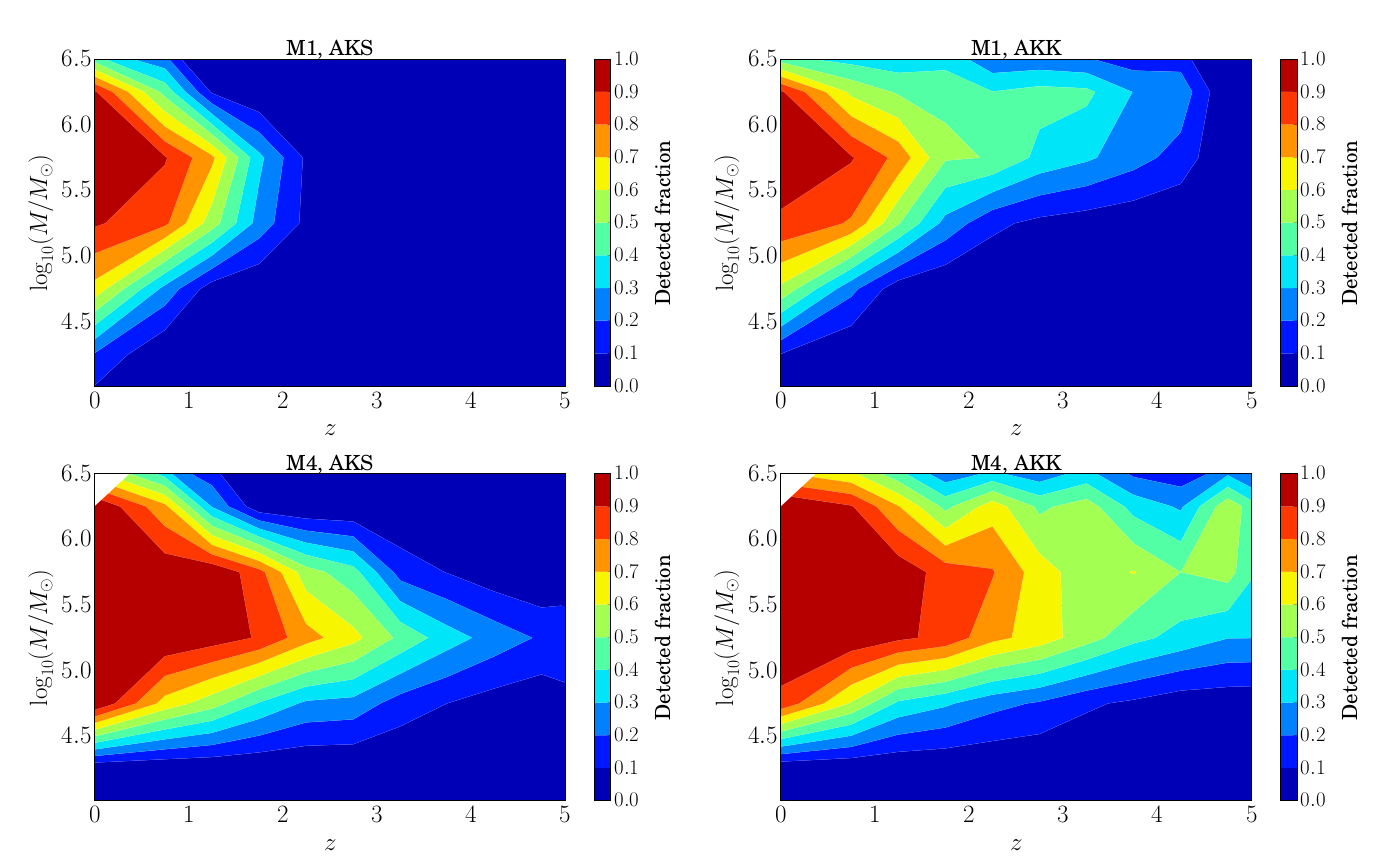
\includegraphics[width=\textwidth]{img/detection_fraction.png}

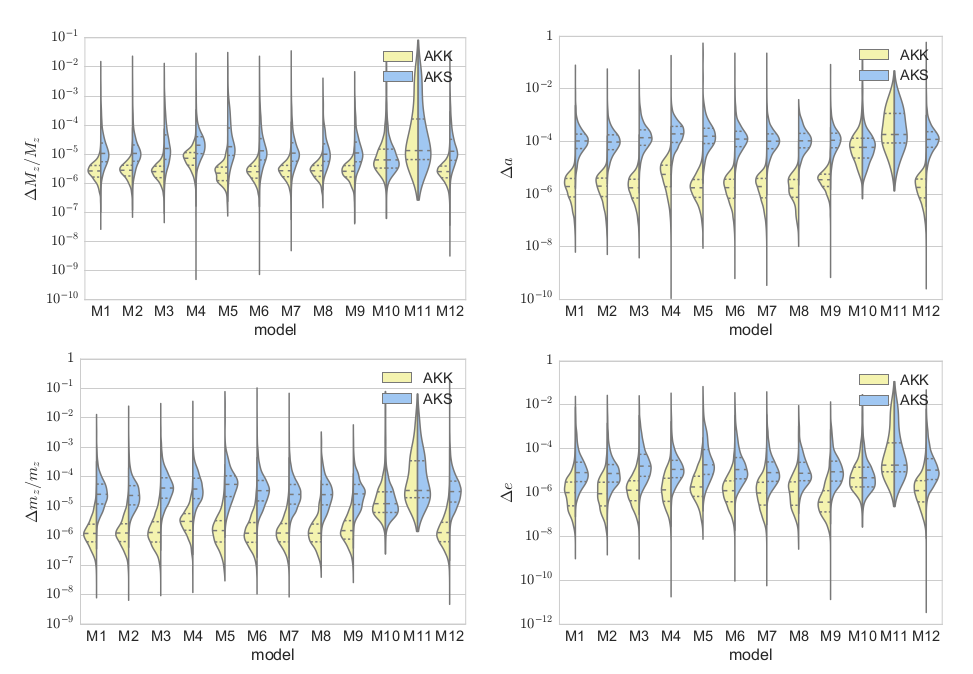
\includegraphics[width=\textwidth]{img/intristic_parameter_estimation.png}

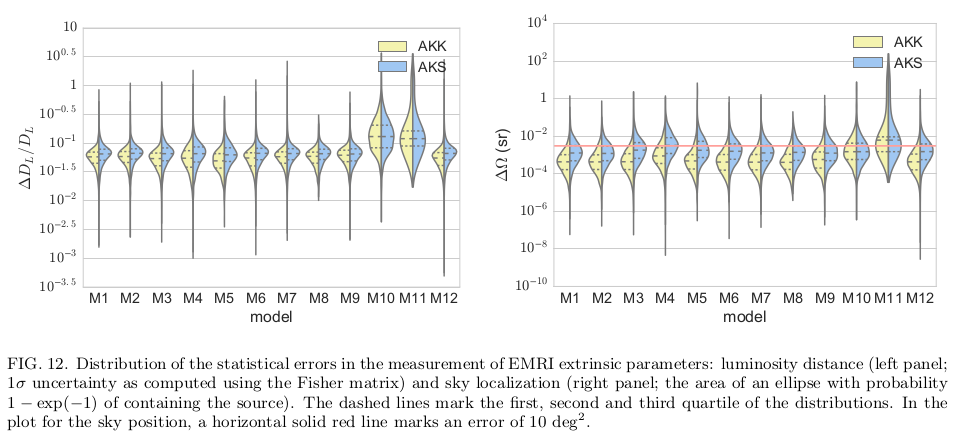
\includegraphics[width=\textwidth]{img/extrinsic_parameter_estimation.png}

\section{Phys. Rev. D 95, 103012}
intrinsic parameters can be recovered with an error of $\approx 10^{-6} -10^{-4}$.
Luminosity distance $\approx 10\%$ and sky localization few deg$^2$.
